% SLIDE 8: Quy Trình Phát Triển dự án
\section{V. Giải Pháp Và Công Nghệ}

\begin{frame}
\frametitle{Điểm yếu của Saboteur}
\begin{columns}
    \column{0.05\textwidth}
    \column{0.4\textwidth}
    \begin{block}{Saboteur có 1 điểm yếu}
        Vai trò của của \textbf{Kẻ phá hoại} sẽ dễ bị lộ, thường chỉ sau nửa game.
    \end{block}
    \column{0.1\textwidth}
    \column{0.4\textwidth}
    \begin{block}{Giải pháp}
        Sáng tạo ra một biến thể mới cho Saboteur với nhiều sự hỗn loạn hơn.
    \end{block}
    \column{0.05\textwidth}
\end{columns}
\end{frame}

% New Saboteur
% 11
\begin{frame}
\frametitle{Sáng tạo luật chơi mới - Biến thể Saboteur với  ngày đêm}
    \begin{figure}[H]
        \centering
        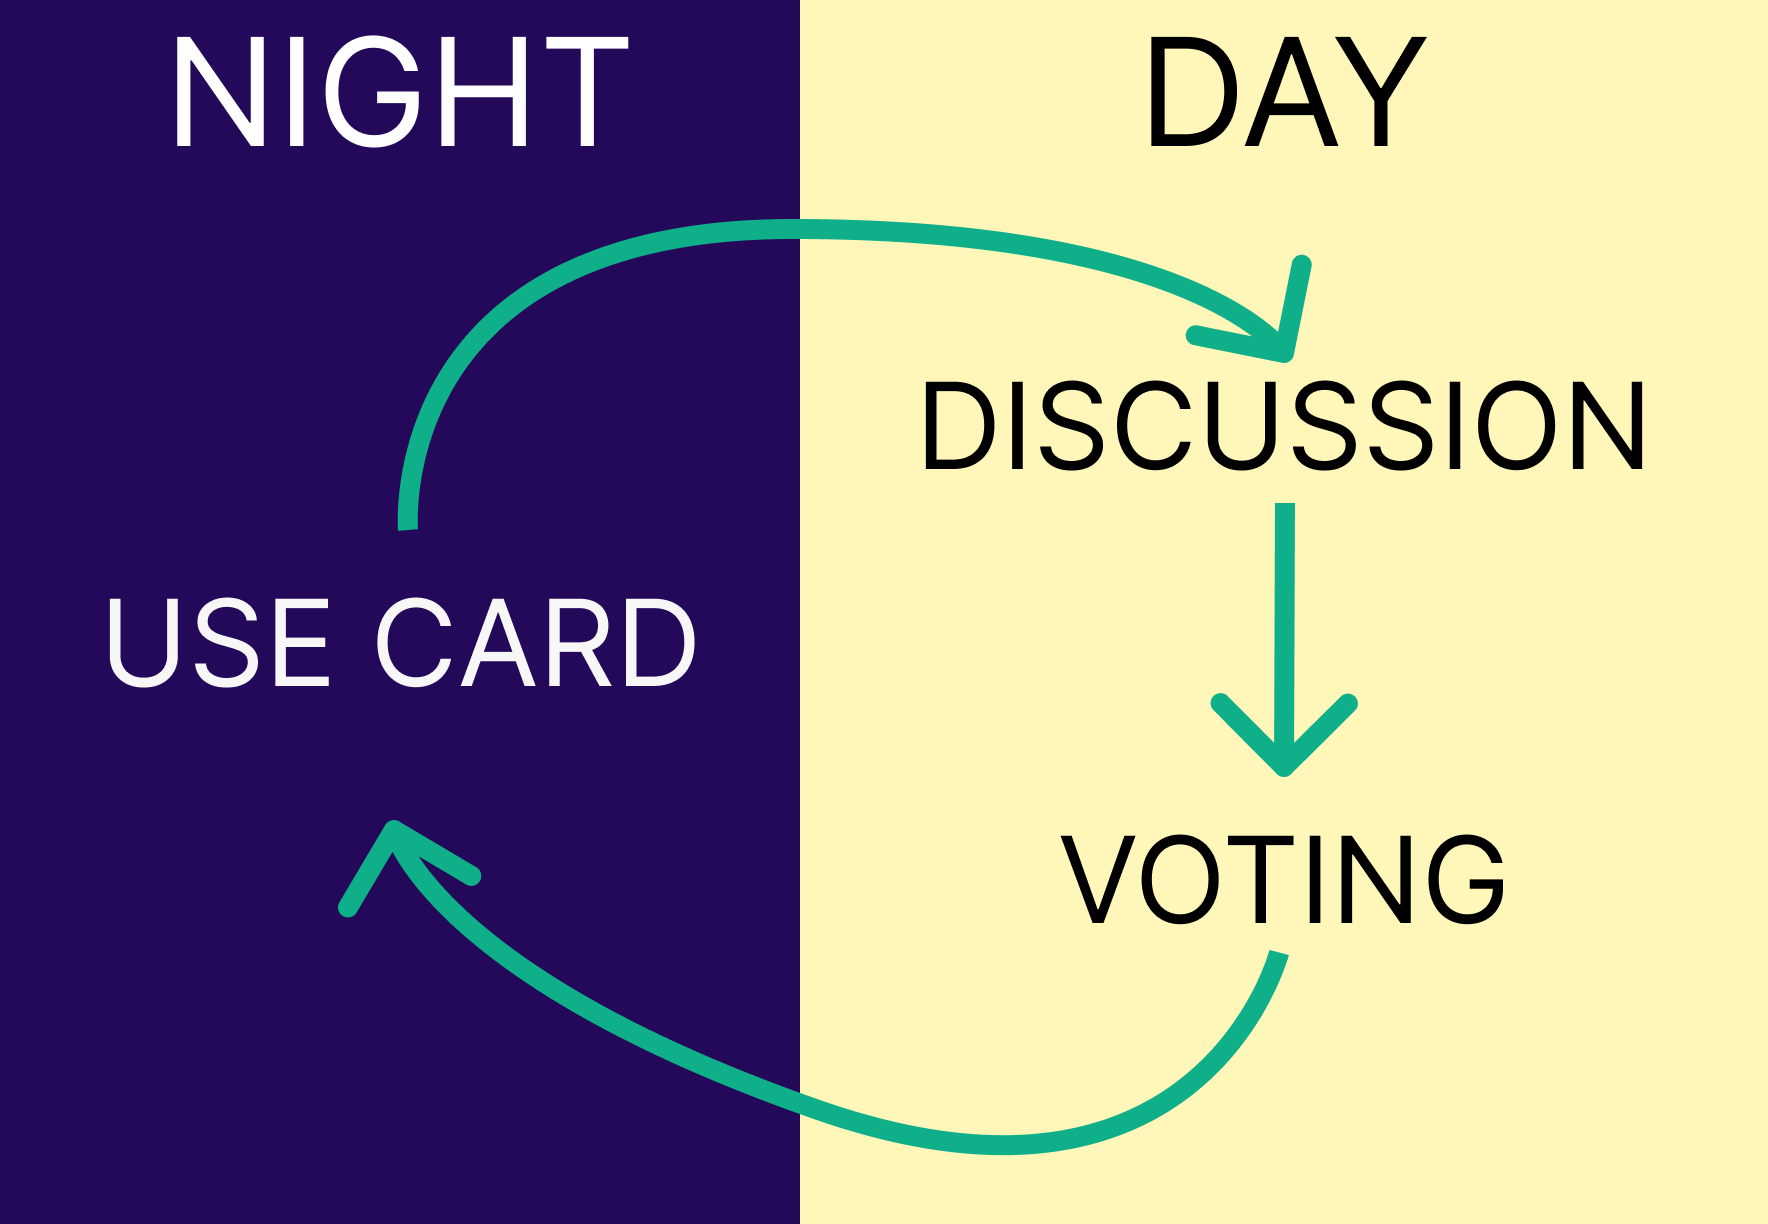
\includegraphics[width=0.5\linewidth]{saboteur/day-night.png}
    \end{figure}
\centering
Mỗi round được chia thành hai pha chính: \textbf{Đêm} và \textbf{Ngày}.
\end{frame}


\begin{frame}
\frametitle{Cấu trúc một Round (Day - Night)}
\begin{columns}
    \column{0.49\textwidth}
    \textbf{Đêm (Night Phase)}
    \begin{itemize}
        \item Bản đồ tối, chỉ người chơi hiện tại nhìn thấy
        \item Thứ tự lượt chơi \textbf{ngẫu nhiên}
        \item Mỗi người chơi có \textbf{15--30 giây} để:
        \begin{itemize}
            \item Đặt thẻ đường / dùng thẻ hành động
            \item Bốc bài
        \end{itemize}
        \item Hoàn thành lượt → Bản đồ tối lại
    \end{itemize}

    \column{0.02\textwidth}
    \centering
    \rule{0.5pt}{0.6\textheight}   % Đường thẳng phân cách

    \column{0.49\textwidth}
    \textbf{Ngày (Day Phase)}
    \begin{itemize}
        \item Bản đồ sáng hoàn toàn, mọi người cùng nhìn thấy thay đổi
        \item \textbf{60 giây} để trò chuyện, tranh luận, đọc vị
        \item Cuối pha: \textbf{Bỏ phiếu}
        \begin{itemize}
            \item Vote \textbf{skip} hoặc vote người chơi
            \item Người bị vote nhiều nhất \textbf{bị cấm hành động} ở Đêm sau
        \end{itemize}
    \end{itemize}
\end{columns}
\end{frame}

\begin{frame}
\frametitle{Cấu trúc một Round (Day)}
    \begin{figure}[H]
        \centering
        \includegraphics[width=0.8\linewidth]{saboteur/day-night-cycle.png}
    \end{figure}
\end{frame}

\begin{frame}
\frametitle{Cấu trúc một Round (Night)}
    \begin{figure}[H]
        \centering
        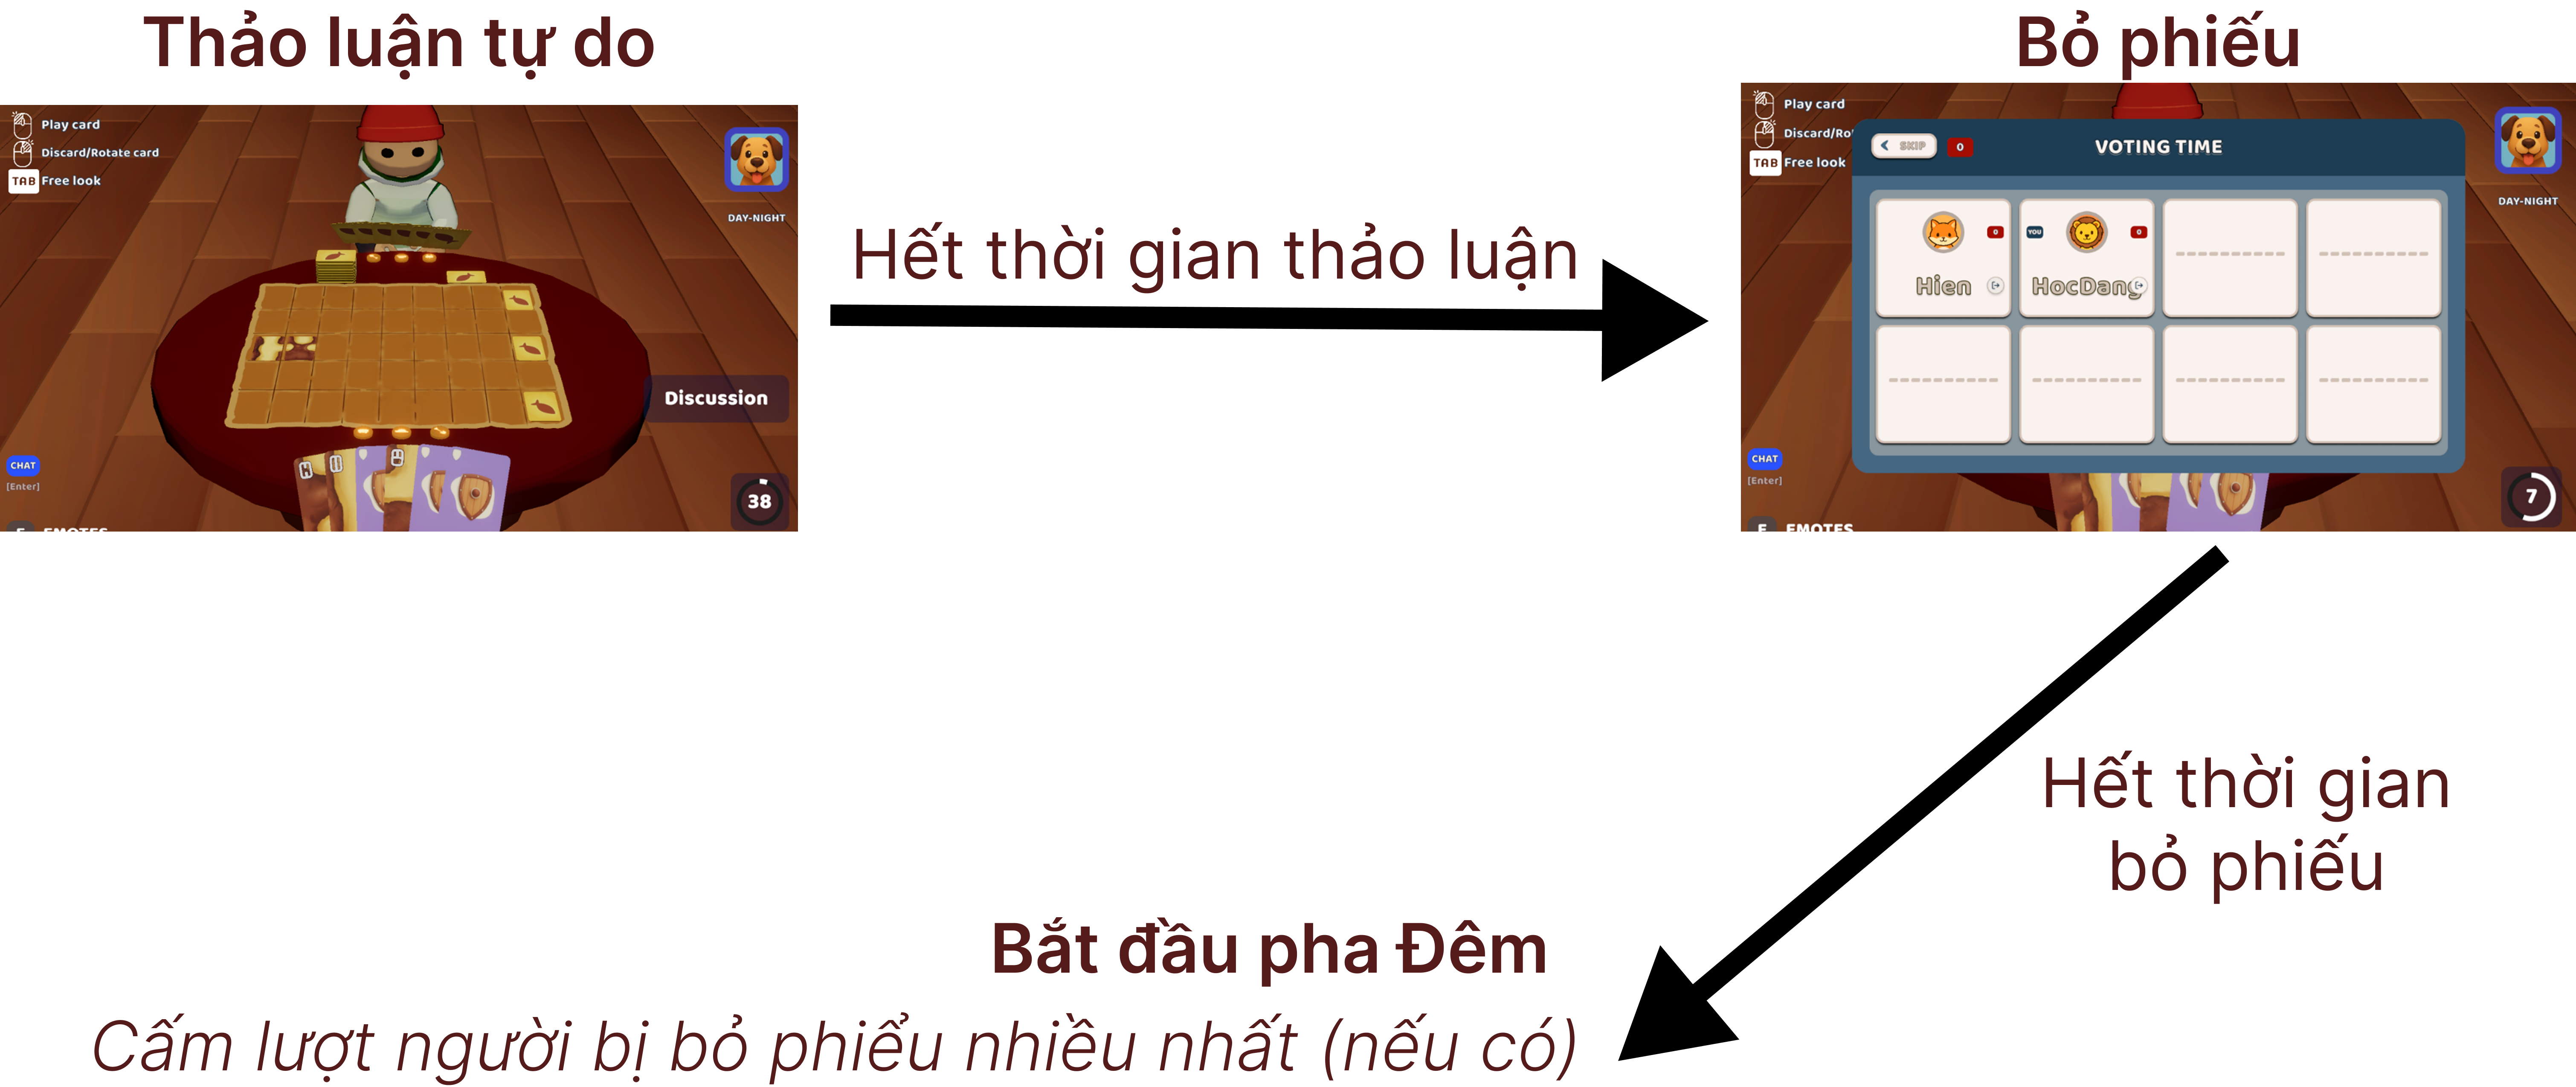
\includegraphics[width=0.8\linewidth]{saboteur/day-cycle.png}
    \end{figure}
\end{frame}

\begin{frame}
\frametitle{Thẻ hành động mới}
\begin{columns}
\column{0.33\textwidth}
    \begin{figure}[H]
        \centering
        
\includegraphics[width=0.4\linewidth]{saboteur/Card_Binoculars_S.png}
    \end{figure}
    \begin{itemize}
        \item Nhìn thấy toàn bộ bản đồ từ lúc chơi thẻ cho đến hết \textbf{Đêm} hiện tại.
    \end{itemize}
\column{0.33\textwidth}
    \begin{figure}[H]
        \centering
        
\includegraphics[width=0.4\linewidth]{saboteur/Card_Shield_S.png}
    \end{figure}
    \begin{itemize}
        \item Đỡ được 1 đòn tấn công phá công cụ. Không tích lũy
    \end{itemize}

\column{0.33\textwidth}
    \begin{figure}[H]
        \centering
        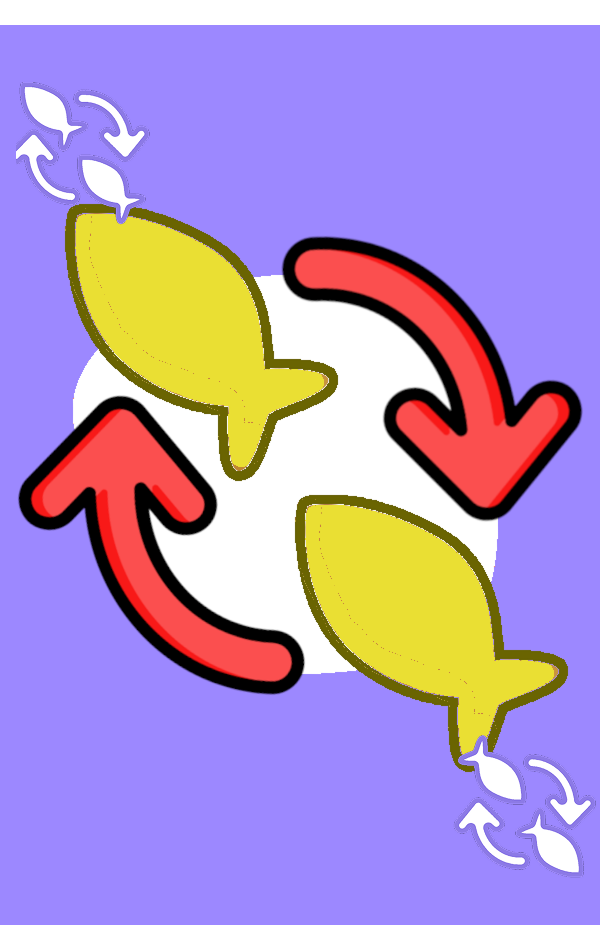
\includegraphics[width=0.4\linewidth]{saboteur/Card_Swap_Goals_S.png}
        % \caption*{Các loại thẻ đường}
    \end{figure}
    \begin{itemize}
        \item Hoán đổi vị trí của 2 trong 3 thẻ Goal (khi chúng vẫn đang úp)
    \end{itemize}
\end{columns}
\end{frame}

% \begin{frame}
% \frametitle{Quy Trình Phát Triển Dự Án}
% \textbf{So sánh các giải pháp:}
% \begin{itemize}
%     \item \textbf{Mô hình Waterfall:} Ổn định nhưng cứng nhắc, khó quay lại giai đoạn trước.
%     \item \textbf{Mô hình sử dụng Agile tự do:} Linh hoạt, tăng cường làm việc nhóm nhưng khó kiểm soát tiến độ.
%     \item \textbf{Mô hình Scrum:} Chia nhỏ giai đoạn (Sprint), sản phẩm hoàn thiện sau mỗi chu kỳ.
% \end{itemize}
% \vspace{0.5cm}
% \textbf{Lựa chọn: Mô hình Scrum}
% \begin{itemize}
%     \item Phù hợp với khung thời gian cố định và yêu cầu làm việc nhóm của đồ án.
%     \item Quản lý tiến độ chặt chẽ qua từng Sprint (2 tuần).
% \end{itemize}
% \end{frame}

% SLIDE 9: Công Cụ Hỗ Trợ
% \begin{frame}
% \frametitle{Công Cụ Hỗ Trợ}
% \begin{itemize}
%     \item \textbf{Discord:} Giao tiếp, họp nhóm và chia sẻ tài nguyên nhanh.
%     \item \textbf{Git \& GitHub:} Quản lý mã nguồn phân tán, hỗ trợ làm việc song song (Branch/Merge).
%     \item \textbf{Jira:} Quản lý task (To Do, In Progress, Done) và theo dõi tiến độ Sprint theo mô hình Scrum.
% \end{itemize}

% \begin{figure}[htbp]
%      \centering
%      % Hình thứ nhất
%      \begin{subfigure}[b]{0.2\textwidth}
%          \centering
%         
\includegraphics[width=\textwidth]{img/Discord.png}
%          \label{fig:discord}
%      \end{subfigure}
%      \hfill % Tạo khoảng trống giữa các hình
%      % Hình thứ hai
%      \begin{subfigure}[b]{0.2\textwidth}
%          \centering
%         
\includegraphics[width=\textwidth]{img/Git.png}
%          \label{fig:git}
%      \end{subfigure}
%      \hfill
%      \begin{subfigure}[b]{0.2\textwidth}
%          \centering
%         
\includegraphics[width=\textwidth]{img/Github.png}
%          \label{fig:github}
%      \end{subfigure}
%      \hfill
%      \begin{subfigure}[b]{0.2\textwidth}
%          \centering
%         
\includegraphics[width=\textwidth]{img/Jira.png}
%          \label{fig:jira}
%      \end{subfigure}
%      \label{fig:three_graphs}
% \end{figure}
% \end{frame}

% SLIDE 10: Game Engine
\begin{frame}
\frametitle{Game Engine}
\textbf{So sánh:}
\begin{itemize}
    \item \textbf{Unreal Engine:} Đồ họa AAA, dùng C++/Blueprint, nhưng nặng và phức tạp.
    \item \textbf{Godot:} Mã nguồn mở, nhẹ, miễn phí, nhưng cộng đồng nhỏ hơn.
    \item \textbf{Unity:} Hỗ trợ đa nền tảng mạnh mẽ, cộng đồng lớn, dùng C\#.
\end{itemize}
\begin{figure}[htbp]
     \centering
     % Hình thứ nhất
     \begin{subfigure}[b]{0.3\textwidth}
         \centering
        
\includegraphics[width=\textwidth]{img/Unreal.png}
         \label{fig:unreal}
     \end{subfigure}
     \hfill % Tạo khoảng trống giữa các hình
     % Hình thứ hai
     \begin{subfigure}[b]{0.3\textwidth}
         \centering
        
\includegraphics[width=\textwidth]{img/Godot.png}
         \label{fig:godot}
     \end{subfigure}
     \hfill
     \begin{subfigure}[b]{0.3\textwidth}
         \centering
        
\includegraphics[width=\textwidth]{img/Unity.png}
         \label{fig:unity}
     \end{subfigure}
     \label{fig:engine}
\end{figure}
\textbf{Lựa chọn: Unity 6}
\begin{itemize}
    \item Cân bằng giữa hiệu năng và tính dễ sử dụng của ngôn ngữ C\#.
    \item Hệ sinh thái hỗ trợ Multiplayer (Netcode, Vivox) phong phú, phù hợp quy mô, mục tiêu dự án.
\end{itemize}
\end{frame}

% SLIDE 11: So Sánh Giải Pháp Netcode
\begin{frame}
\frametitle{Các Giải Pháp Netcode}
\textbf{So sánh:}
\begin{itemize}
    \item \textbf{Photon (PUN/Fusion):} Dễ dùng nhưng chi phí cao khi scale.
    \item \textbf{Mirror:} Mã nguồn mở, miễn phí nhưng cần tự xử lý logic server phức tạp.
    \item \textbf{Netcode for GameObjects (NGO):} Giải pháp chính chủ, khuyến nghị của Unity.
\end{itemize}
\begin{figure}[htbp]
     \centering
     % Hình thứ nhất
     \begin{subfigure}[b]{0.3\textwidth}
         \centering
        
\includegraphics[width=\textwidth]{img/Photon.jpg}
         \label{fig:photon}
     \end{subfigure}
     \hfill % Tạo khoảng trống giữa các hình
     % Hình thứ hai
     \begin{subfigure}[b]{0.2\textwidth}
         \centering
        
\includegraphics[width=\textwidth]{img/mirror.jpg}
         \label{fig:mirror}
     \end{subfigure}
     \hfill
     \begin{subfigure}[b]{0.3\textwidth}
         \centering
        
\includegraphics[width=\textwidth]{img/NGO.png}
         \label{fig:NGO}
     \end{subfigure}
     \label{fig:netcode}
\end{figure}
\textbf{Lựa chọn: Unity NGO}
\begin{itemize}
    \item Giải pháp chính thức, tương thích cao với Unity Services (Relay, Lobby).
    \item Miễn phí cho quy mô nhỏ (<50 CCU), phù hợp dự án học thuật.
\end{itemize}
\end{frame}

% SLIDE 12: So Sánh Kiến Trúc Mạng
\begin{frame}
\frametitle{Các Kiến Trúc Mạng}
\textbf{Mô hình:}
\begin{itemize}
    \item \textbf{Client-Server (Dedicated):} Ổn định, công bằng, bảo mật cao nhưng tốn chi phí server.
    \item \textbf{Client-Host:} Một người chơi làm máy chủ, đơn giản, tiết kiệm chi phí.
\end{itemize}
\vspace{0.5cm}
\textbf{Lựa chọn: Client-Host}
\begin{itemize}
    \item Tối ưu tốc độ phát triển và chi phí (không cần thuê server).
    \item Phù hợp thử nghiệm gameplay, dễ debug.
    \item \textit{Định hướng trong tương lai:} Chuyển sang Dedicated Server để tăng ổn định.
\end{itemize}
\end{frame}

% SLIDE 13: Hệ Thống Voice-Text Chat
\begin{frame}
\frametitle{Hệ Thống Voice-Text Chat: Vivox}
\textbf{So sánh:}
\begin{itemize}
    \item \textbf{Dissonance:} Tùy biến cao, trả phí (Asset Store), cần tự setup backend.
    \item \textbf{Photon Voice-Chat:} Tốt cho game realtime nhưng thường đi kèm gói trả phí của Photon.
    \item \textbf{Vivox:} Giải pháp chuyên nghiệp, tích hợp sẵn trong Unity Services.
\end{itemize}
\begin{figure}[htbp]
     \centering
     \begin{subfigure}[b]{0.2\textwidth}
         \centering
        
\includegraphics[width=\textwidth]{img/dissonance.jpg}
         \label{fig:dissonance}
     \end{subfigure}
     \hfill
     % Hình thứ nhất
     \begin{subfigure}[b]{0.2\textwidth}
         \centering
        
\includegraphics[width=\textwidth]{img/photon-voice.jpg}
         \label{fig:photon-voice}
     \end{subfigure}
     \begin{subfigure}[b]{0.2\textwidth}
         \centering
        
\includegraphics[width=\textwidth]{img/photon-chat.jpg}
         \label{fig:photon-chat}
     \end{subfigure}
     \hfill % Tạo khoảng trống giữa các hình
     % Hình thứ hai
     \begin{subfigure}[b]{0.3\textwidth}
         \centering
        
\includegraphics[width=\textwidth]{img/vivox.jpg}
         \label{fig:vivox}
     \end{subfigure}
     \label{fig:voice-chat}
\end{figure}
\textbf{Lựa chọn: Vivox}
\begin{itemize}
    \item Miễn phí lên đến 5000 PCU, chất lượng âm thanh tốt.
    \item API dễ tích hợp.
    \item Tích hợp text chat nhanh chóng.
\end{itemize}
\end{frame}

% SLIDE 14: Design Patterns Áp Dụng
\begin{frame}
\frametitle{Design Patterns Áp Dụng}
\begin{itemize}
    \item \textbf{Singleton Pattern:}
    \begin{itemize}
        \item Quản lý các hệ thống duy nhất: \texttt{GameManager}, \texttt{NetworkManager}.
        \item Cung cấp điểm truy cập toàn cục tiện lợi.
    \end{itemize}
    
    \item \textbf{Observer Pattern (ScriptableObjects):}
    \begin{itemize}
        \item Dùng Event Channels để giảm sự phụ thuộc (decoupling) giữa các module.
        \item Dễ dàng mở rộng, bảo trì logic game.
    \end{itemize}
    
    \item \textbf{State Pattern:}
    \begin{itemize}
        \item Quản lý trạng thái nhân vật: \texttt{Idle}, \texttt{Move}, \texttt{Jump}.
        \item Tách biệt logic hành vi, dễ dàng thêm trạng thái mới.
    \end{itemize}
\end{itemize}
\end{frame}

\begin{frame}
\frametitle{Kiến Trúc Hệ Thống}
    \begin{figure}[H]
        \centering
        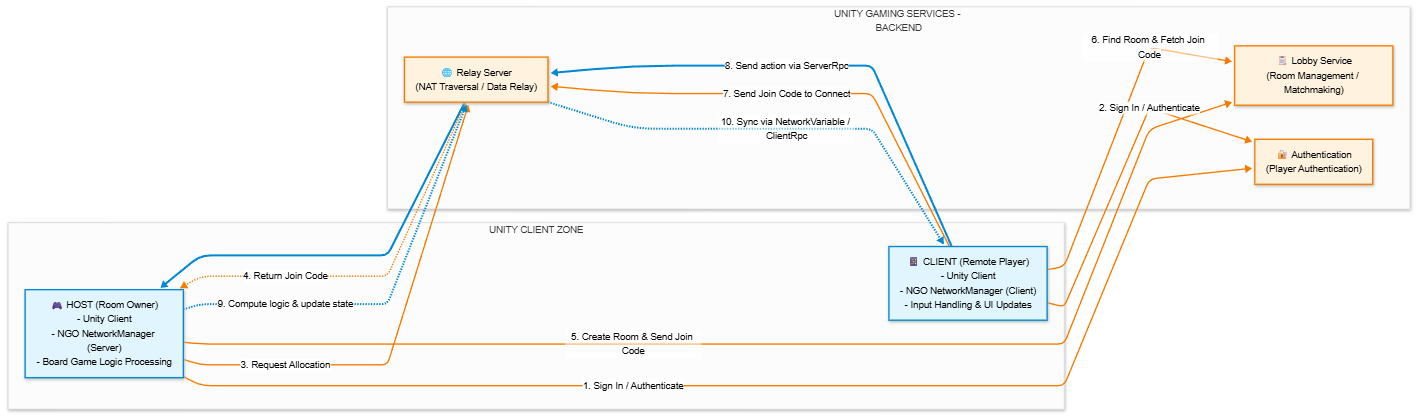
\includegraphics[width=1\linewidth]{diagram/Architecture.png}
    \end{figure}
\end{frame}